\chapter*{Prerequisites to GPT-3}
\label{chap:prereq}
\thispagestyle{fancy}
\addcontentsline{toc}{chapter}{\nameref{chap:prereq}}

\hspace{0.5cm} This seminar covers advanced topics under artificial intelligence. The following sections will engage the reader with some of the basics to AI and sub-fields such as machine learning, neural networks etc. Most of it will be as elucidation of terminologies. The reader is advised to follow up whatever is required for their understanding, please.

\section*{Machine Learning}
\label{sec:mchlrn}
\addcontentsline{toc}{section}{\nameref{sec:mchlrn}}

\hspace{0.5cm} Machine Learning is a sub field of Artificial Intelligence which is a new technique to solve complex problems. Factually the `new technique' is/are set of algorithms which improve automatically through experience. In conventional programming the programmer is responsible for providing the machine with instructions to perform a certain task, as in figure \eqref{fig:clsc_pgm}. But in real world scenario problems are extremely complex to be solved with human generated rules.

\begin{figure}[!htbp]
    \centering
    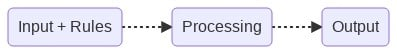
\includegraphics[width=0.7\textwidth]{classical.jpeg}
    \caption[Classical Programming]{Classical Programming}
    \label{fig:clsc_pgm}
\end{figure}

In machine learning the programmers supply the system with data and the expected output as input examples during training \cite{devto:urfstai}, as in figure \eqref{fig:mltrain}. During training period the machine improves in the tasks at hand gradually.

\begin{figure}[!htbp]
    \centering
    \begin{minipage}{0.45\textwidth}
        \centering
        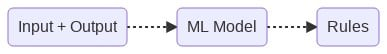
\includegraphics[width=\textwidth]{ml_train.jpeg}
        \caption[ML Training]{\centering ML Training }
        \label{fig:mltrain}
    \end{minipage}\hfill
    \begin{minipage}{0.45\textwidth}
        \centering
        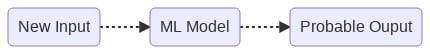
\includegraphics[width=\textwidth]{ml_test.jpeg}
        \caption[ML Testing]{\centering ML Testing}
        \label{fig:mltest}
    \end{minipage}
\end{figure}

When the machine learning `model' is ready to map similar input output without humans explicitly defining each and every one of them, it enters the testing phase. The models is tested on some data which it has never seen before and predicts the output as shown in figure \eqref{fig:mltest}. There are various types of machine learning algorithms like: Supervised, Unsupervised adn Reinforced learning. Deep Learning is a subset of Machine Learning and it is called so because of the deep structure of the underlying architecture. 

\section*{Feed-forward Neural Networks}
\label{sec:ffnn}
\addcontentsline{toc}{section}{\nameref{sec:ffnn}}
\hspace{0.5cm} A feed-forward neural network is an artificial neural network wherein connections between the nodes do not form a cycle. The feed-forward neural network was the first and simplest type of artificial neural network devised. In this network, the information moves in only one direction—forward—from the input nodes, through the hidden nodes (if any) and to the output nodes. There are no cycles or loops in the network.

The simplest kind of neural network is a single-layer perceptron network, which consists of a single layer of output nodes; the inputs are fed directly to the outputs via a series of weights. The sum of the products of the weights and the inputs is calculated in each node, and if the value is above some threshold (typically 0) the neuron fires and takes the activated value (typically 1); otherwise it takes the deactivated value (typically -1) \cite{wiki:ffnn}. 

\section*{Activation Function}
\label{sec:actvfnc}
\addcontentsline{toc}{section}{\nameref{sec:actvfnc}}
In artificial neural networks, the activation function of a node defines the output of that node given an input or set of inputs. A standard integrated circuit can be seen as a digital network of activation functions that can be `ON' or `OFF', depending on input. A single-layer neural network can compute a continuous output instead of a step function. A common choice is the so-called logistic function:

\[f(x) = \frac{1}{1+e^{-x}}\]

The most common activation functions can be divided in three categories: ridge functions, radial functions and fold functions. Ridge functions are univariate functions acting on a linear combination of the input variables. Often used examples include, Linear: $\phi(v) = a + v'b$, ReLU $\phi(v) = max(0, a + v'b)$ etc. In multiclass classification the \emph{softmax} activation is often used \cite{wiki:actvfnc}.

\section*{Natural Language Processing}
\label{sec:nlp}
\addcontentsline{toc}{section}{\nameref{sec:nlp}}

Natural language processing (NLP) is concerned with the interactions between computers and human language, in particular how to program computers to process and analyze large amounts of natural language data. The result is a computer capable of ‘understanding’ the contents of documents, including the contextual nuances of the language within them. The technology can then accurately extract information and insights contained in the documents as well as categorize and organize the documents themselves.

Challenges in natural language processing frequently involve speech recognition, natural language understanding, and natural-language generation \cite{wiki:nlp}. 

\section*{Language Models}
\label{sec:langmodls}
\addcontentsline{toc}{section}{\nameref{sec:langmodls}}

\hspace{0.5cm} A statistical language model is a probability distribution over sequences of words. Given such a sequence, say of length $m$, it assigns a probability $P(w_1, \dots, w_m)$ to the whole sequence. The language model provides context to distinguish between words and phrases that sound similar. Data sparsity is a major problem in building language models. Most possible word sequences are not observed in \emph{training}. One solution is to make the assumption that the probability of a word only depends on the previous $n$ words. This is known as an $n$-gram model or unigram model when $n = 1$. The unigram model is also known as the \emph{bag of words model} \cite{wiki:langmdl}.

\section*{Transfer Learning}
\label{sec:trnsfrlrn}
\addcontentsline{toc}{section}{\nameref{sec:trnsfrlrn}}

\hspace{0.5cm} Transfer learning (TL) is a research problem in machine learning (ML) that focuses on storing knowledge gained while solving one problem and applying it to a different but related problem. For example, knowledge gained while learning to recognize cars could apply when trying to recognize trucks. This area of research bears some relation to the long history of psychological literature on transfer of learning.

From the practical standpoint, reusing or transferring information from previously learned tasks for the learning of new tasks has the potential to significantly improve the sample efficiency of a reinforcement learning agent. Given a source domain $D_S$ and learning task $T_S$, a target domain $D_T$ and learning task $T_T$, where $D_S \neq D_T$, or $T_S \neq T_T$, transfer learning aims to help improve the learning of the target predictive function $f_T(\cdot)$ in $T_T$ using the knowledge in $D_S$ and $T_S$ \cite{wiki:trnsflrn}.

\begin{figure}[!htbp]
    \centering
    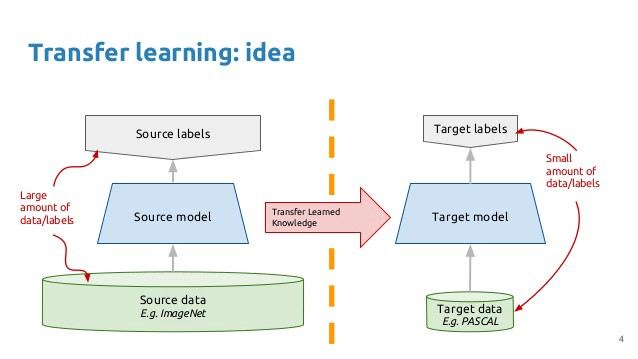
\includegraphics[width=0.9\textwidth]{transfer_learning.jpeg}
    \caption[Transfer Learning]{Transfer Learning}
    \label{fig:trnsflrnimg}
\end{figure}

\vspace*{\fill}